\documentclass[12pt]{article}
\usepackage[margin=1in]{geometry}
\usepackage{graphicx}
\usepackage{amsmath}
\usepackage{lscape}
\usepackage{fancyhdr}
\usepackage{hyperref}
\usepackage{booktabs}

% Setup header
\pagestyle{fancy}
\fancyhf{}
\fancyhead[L]{USC Facilities: Rain Barrel Water Pump System} % Team name in the header
\fancyfoot[C]{\thepage} % Page number in the footer


\title{
    \vspace{2in}
    \textbf{EMCH427-002} \\[1ex]
    \textbf{Product Specifications Report} \\[1ex]
    \textbf{Sponsor: USC Facilities} \\[1ex]
    \vspace{2in}
}

\author{
    \textbf{Team Members:} \\[2ex]
    Tanner Harmon -- Compiled the Report and Wrote Introduction/Conclusion \\[1ex]
    Presston McConnell -- Managed Competitor Analysis \\[1ex]
    William Wenzel --  Developed the Needs Metrics Matrix \\[1ex]
    Jacob Vaught -- Handled Target and Fallback Specifications  \\[2ex]
    \textbf{Note:} All team members contributed to the appendix.
}

\date{}

\maketitle
\thispagestyle{fancy}

\newpage
\section{Introduction}

\begin{itemize}
    \item \textbf{Context:}
    \begin{itemize}
        \item Water conservation and sustainable landscaping are critical concerns for the University of South Carolina (USC) Facilities department.
        \item USC Facilities initiated a project to design and implement a Rain Barrel Water Pump System for irrigating campus gardens using collected rainwater.
    \end{itemize}
    
    \item \textbf{Project Aims:}
    \begin{itemize}
        \item Reduce potable water usage.
        \item Promote environmental sustainability.
        \item Enhance the efficiency of garden maintenance operations.
    \end{itemize}
    
    \item \textbf{Primary Goal:}
    \begin{itemize}
        \item Develop a reliable, user-friendly, and efficient water pump system using stored rainwater for campus garden irrigation.
    \end{itemize}
    
    \item \textbf{Key Challenges:}
    \begin{itemize}
        \item Ensuring sufficient water pressure and flow rate for effective irrigation.
        \item Minimizing manual labor and operational effort for maintenance staff.
        \item Integrating the system seamlessly into the landscape without posing safety risks.
    \end{itemize}
    
    \item \textbf{Design Alignment:}
    \begin{itemize}
        \item A comprehensive process was undertaken to identify, prioritize, and translate customer needs into measurable engineering specifications.
        \item The system must meet the needs and expectations of USC Facilities and the end-users (garden maintenance staff and the campus community).
    \end{itemize}
    
    \item \textbf{Methodology:}
    \begin{itemize}
        \item The House of Quality (HoQ) methodology, part of Quality Function Deployment (QFD), was used to capture customer requirements systematically.
        \item Importance of customer needs was assessed, and target specifications for the system's technical features were established.
    \end{itemize}
    
    \item \textbf{HoQ Rationale:}
    \begin{itemize}
        \item HoQ bridges the gap between customer desires and engineering realities.
        \item Facilitates a structured decision-making process that prioritizes features based on customer satisfaction.
        \item Focuses design efforts on delivering maximum value to USC Facilities while efficiently allocating resources to critical aspects.
    \end{itemize}
\end{itemize}


\newpage
\section{Needs Metrics}

\subsection{Customer Needs Identification and Reduction}

\subsubsection{Initial Customer Needs Collection}

An extensive needs-gathering process was conducted, involving interviews with USC Facilities personnel, garden maintenance staff, and other stakeholders. This process resulted in the identification of 140 initial Customer Needs and Requirements (CNRs), covering a wide range of aspects from operational efficiency to environmental impact.

\subsubsection{Needs Reduction Process}

To make the project manageable and focus on the most critical requirements, a systematic needs reduction process was undertaken. The steps involved were:

\begin{itemize}
    \item \textbf{Grouping Similar Needs:} Similar or overlapping needs were grouped under broader categories to eliminate redundancy. For example, multiple needs related to minimizing manual labor were consolidated.
    \item \textbf{Prioritization Based on Stakeholder Input:} Stakeholders were consulted to rank the importance of each need. Needs that received low importance ratings were considered for exclusion.
    \item \textbf{Feasibility Analysis:} Needs were evaluated for technical and economic feasibility. Needs that were deemed infeasible within the project constraints were deprioritized.
    \item \textbf{Alignment with Project Goals:} Needs were assessed for alignment with the primary project goals of water conservation, operational efficiency, and sustainability.
\end{itemize}

Through this process, the list was reduced from 140 to 24 customer needs in the second round. Further refinement, involving detailed discussions with stakeholders and analysis of potential impact, resulted in a final list of 21 customer needs to be addressed in the preliminary design phase.

\subsection{Justification for Excluded Customer Needs}

The following customer needs were excluded from the preliminary design phase after careful consideration:

\begin{itemize}
    \item \textbf{The system should minimize the physical effort required to operate it.}

    \textbf{Justification:} This need was determined to be implicitly addressed by existing needs focused on minimizing manual labor and operational effort (e.g., "The system should require minimal manual operations" and "The system should be easy to use"). Including it separately was found to be redundant. The design team will ensure that physical effort considerations are encompassed within the broader usability requirements.

    \textbf{Potential Impact:} Excluding this need as a separate item does not negatively impact the design, as its essence is captured within other prioritized needs. Vigilance will be maintained to avoid overlooking any specific aspects related to physical effort.

    \item \textbf{The system should use materials that are safe for plant and human interaction.}

    \textbf{Justification:} This need was consolidated under the broader environmental impact and safety needs, specifically "The system should have minimal environmental impact" and "The system should be safe to operate." By integrating material safety into these broader categories, comprehensive coverage of safety and environmental concerns is ensured without fragmenting the requirements.

    \textbf{Potential Impact:} There is a risk that specific material safety considerations could be diluted within broader categories. To mitigate this, the design specifications for environmental impact and safety will explicitly include material safety criteria.

    \item \textbf{The system should not pose any risks to pedestrians or garden users.}

    \textbf{Justification:} This need is inherently addressed within the overarching safety requirements. The need "The system should be safe to operate and maintain" encompasses safety for all users, including pedestrians and garden visitors. Including this need separately was deemed redundant.

    \textbf{Potential Impact:} Excluding this specific need might lead to less emphasis on pedestrian safety. To prevent this, the safety requirements will be detailed to include risks to all potential users, ensuring comprehensive safety considerations.

\end{itemize}

\subsection{CNR Metrics}

\subsection{Observations and Analysis}

Based on the customer needs and their associated metrics, several critical insights were identified:

\begin{itemize}
    \item \textbf{High Impact Customer Needs:}

    The customer need "The system should provide sufficient water pressure" has a high importance rating and is measured by multiple metrics, including "Water Transfer Rate (L/min)" and "Water Pressure (kPa)." This indicates that achieving adequate water pressure is paramount and will significantly influence the design.

    \item \textbf{Engineering Characteristics with Multiple Metrics:}

    Metrics such as "Flow Rate Consistency (\%)" and "Water Transfer Rate (L/min)" are associated with several customer needs, highlighting their importance. For example, they impact both "The system should distribute water consistently" and "The system should minimize water waste."

    \item \textbf{Overlapping Metrics Indicating Complexity:}

    The customer need "The system should be easy to use" is measured by "Learning Time (hours)" and "User Error Rate (\%)." These metrics suggest that designing for usability will require careful consideration of user interface design and operational simplicity.

    \item \textbf{Sustainability Considerations:}

    Metrics like "Eco-Friendly Materials (\%)" and "Potable Water Savings (liters/month)" emphasize the project's focus on environmental impact. Maximizing these metrics aligns with USC's sustainability goals and offers opportunities for innovation in material selection and water management.

\end{itemize}
\begin{table}[h!]
    \centering
    \caption{Customer Needs and Their Metrics}
    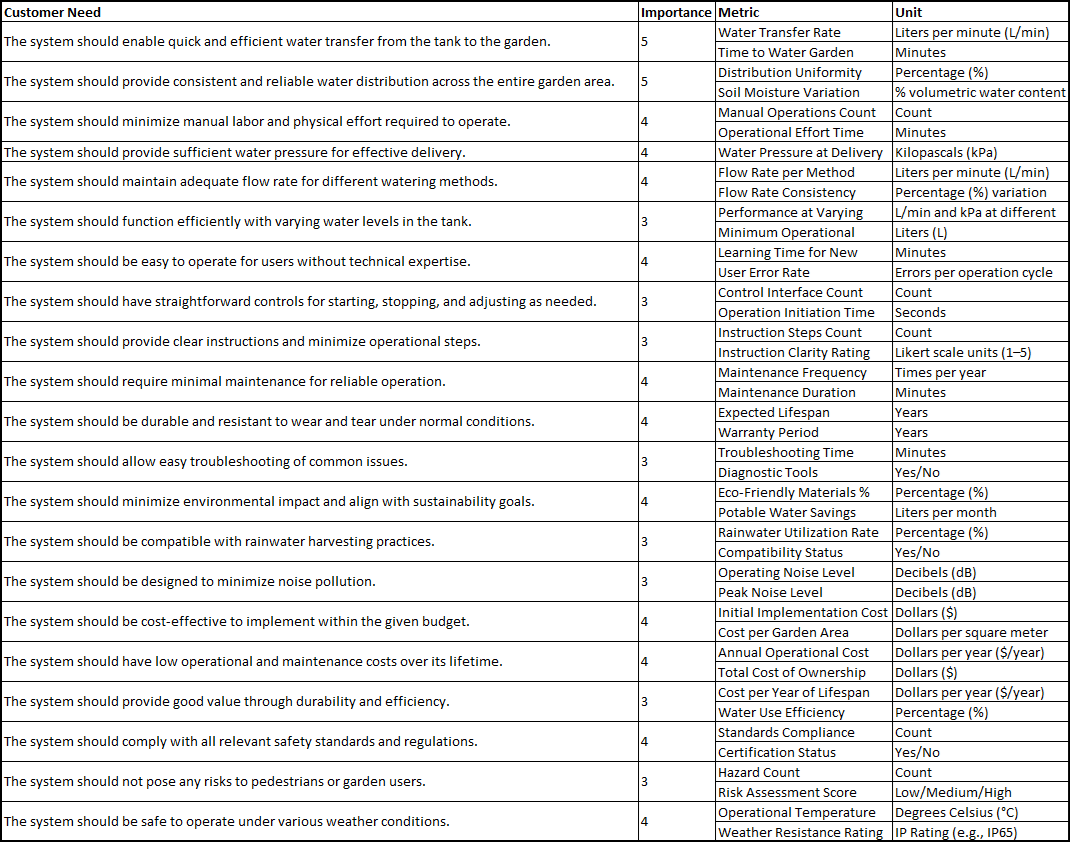
\includegraphics[width=\linewidth]{Cr_to_TR.png}
\end{table}

\newpage
\section{Needs Metrics Matrix}

\subsection{Methodology}

The House of Quality (HoQ) is a structured tool within the Quality Function Deployment (QFD) process that translates customer needs (the "Whats") into engineering characteristics (the "Hows"). For this project, the HoQ methodology was applied specifically to align the Rain Barrel Water Pump System's design with the prioritized customer needs identified earlier.

\subsubsection{Assigning Importance Factors}

Each customer need was assigned an \textbf{Importance Factor} on a scale of 1 to 5, with 5 being the most critical. The assignment was based on stakeholder input, emphasizing needs that have the highest impact on user satisfaction and project goals. For example, "The system should provide sufficient water pressure" received an importance factor of 5 due to its critical role in effective irrigation.

\subsubsection{Defining Engineering Characteristics (ECs)}

Specific, measurable Engineering Characteristics were identified to fulfill the customer needs. Each EC was defined with units and measurable parameters, such as "Water Transfer Rate (L/min)" and "Operational Effort Time (minutes)."

\subsubsection{Establishing Relationships in the Matrix}

The relationship matrix was constructed by assessing the strength of the relationship between each customer need and each EC. The scale used was:

\begin{itemize}
    \item \textbf{9 (Strong Relationship):} The EC has a significant impact on fulfilling the customer need.
    \item \textbf{3 (Moderate Relationship):} The EC has a moderate impact.
    \item \textbf{1 (Weak Relationship):} The EC has a minor impact.
    \item \textbf{0 (No Relationship):} The EC does not affect the customer need.
\end{itemize}

The values were assigned based on engineering judgment and analysis of how each EC influences the satisfaction of the customer needs. For instance, "Water Transfer Rate" has a strong relationship (9) with "The system should provide sufficient water pressure."

\subsubsection{Calculating Weight Factors}

The \textbf{Weight Factors} for each EC were calculated by multiplying the Importance Factors of the customer needs by the relationship strength values and summing them for each EC. This process helped prioritize the ECs that have the most significant impact on meeting customer needs.

\subsubsection{Correlation Matrix}

A correlation matrix (the "roof" of the HoQ) was developed to identify interdependencies between ECs. The correlations were marked as:

\begin{itemize}
    \item \textbf{Positive (+):} Improvement in one EC positively affects another.
    \item \textbf{Negative (-):} Improvement in one EC negatively affects another.
    \item \textbf{Strong Positive (++):} Significant positive impact.
    \item \textbf{Strong Negative (--):} Significant negative impact.
\end{itemize}

For example, "Increasing Water Pressure (kPa)" may have a negative correlation with "Minimizing Energy Consumption (kWh)" because achieving higher pressure typically requires more power.

\subsubsection{Competitor Benchmarking}

Competitor products were included in the HoQ to benchmark their performance against the target specifications. Each competitor was evaluated on how well they meet the customer needs, providing insights into market positioning and opportunities for differentiation.

\subsection{Rationale and Insights Gained}

The application of the House of Quality in this project provided several specific benefits:

\begin{itemize}
    \item \textbf{Prioritization of Engineering Efforts:} By quantifying the relationships between customer needs and ECs, it was identified that "Water Transfer Rate" and "Water Pressure" are the most critical ECs. This prioritization allows focus on optimizing these parameters.

    \item \textbf{Identification of Trade-offs:} The correlation matrix revealed potential conflicts between ECs. For instance, achieving high water pressure may conflict with the goal of minimizing energy consumption and operational costs. Recognizing these trade-offs early enables exploration of design solutions that balance these competing requirements.

    \item \textbf{Competitive Analysis:} Benchmarking against competitor products identified gaps in the market, such as the lack of systems that offer both high performance and low environmental impact. This insight guides the design of a system that differentiates itself by addressing these unmet needs.

    \item \textbf{Stakeholder Alignment:} The HoQ facilitated clear communication with stakeholders by providing a visual representation of how customer needs translate into technical specifications. This alignment ensures that all team members and stakeholders have a shared understanding of project priorities.

\end{itemize}

\subsubsection{Challenges and Limitations Encountered}

While the HoQ methodology provided valuable insights, several challenges were encountered:

\begin{itemize}
    \item \textbf{Complexity in Assigning Relationships:} Determining the strength of relationships between customer needs and ECs required careful consideration and, in some cases, subjective judgment. To mitigate this, team discussions were held to reach consensus on the assignments.

    \item \textbf{Balancing Conflicting Requirements:} The identification of negative correlations highlighted the difficulty in simultaneously optimizing certain ECs. For example, increasing pump power to achieve higher pressure conflicts with the need to minimize energy consumption. Addressing these conflicts will require innovative design solutions and possible compromises.

    \item \textbf{Data Availability for Benchmarking:} Obtaining detailed technical data on competitor products was challenging due to limited publicly available information. Manufacturer specifications were relied upon, and where necessary, values were estimated based on similar products.

\end{itemize}

\subsection{Needs Metrics Matrix Figures Explained}

\begin{figure}[h!]
    \centering
    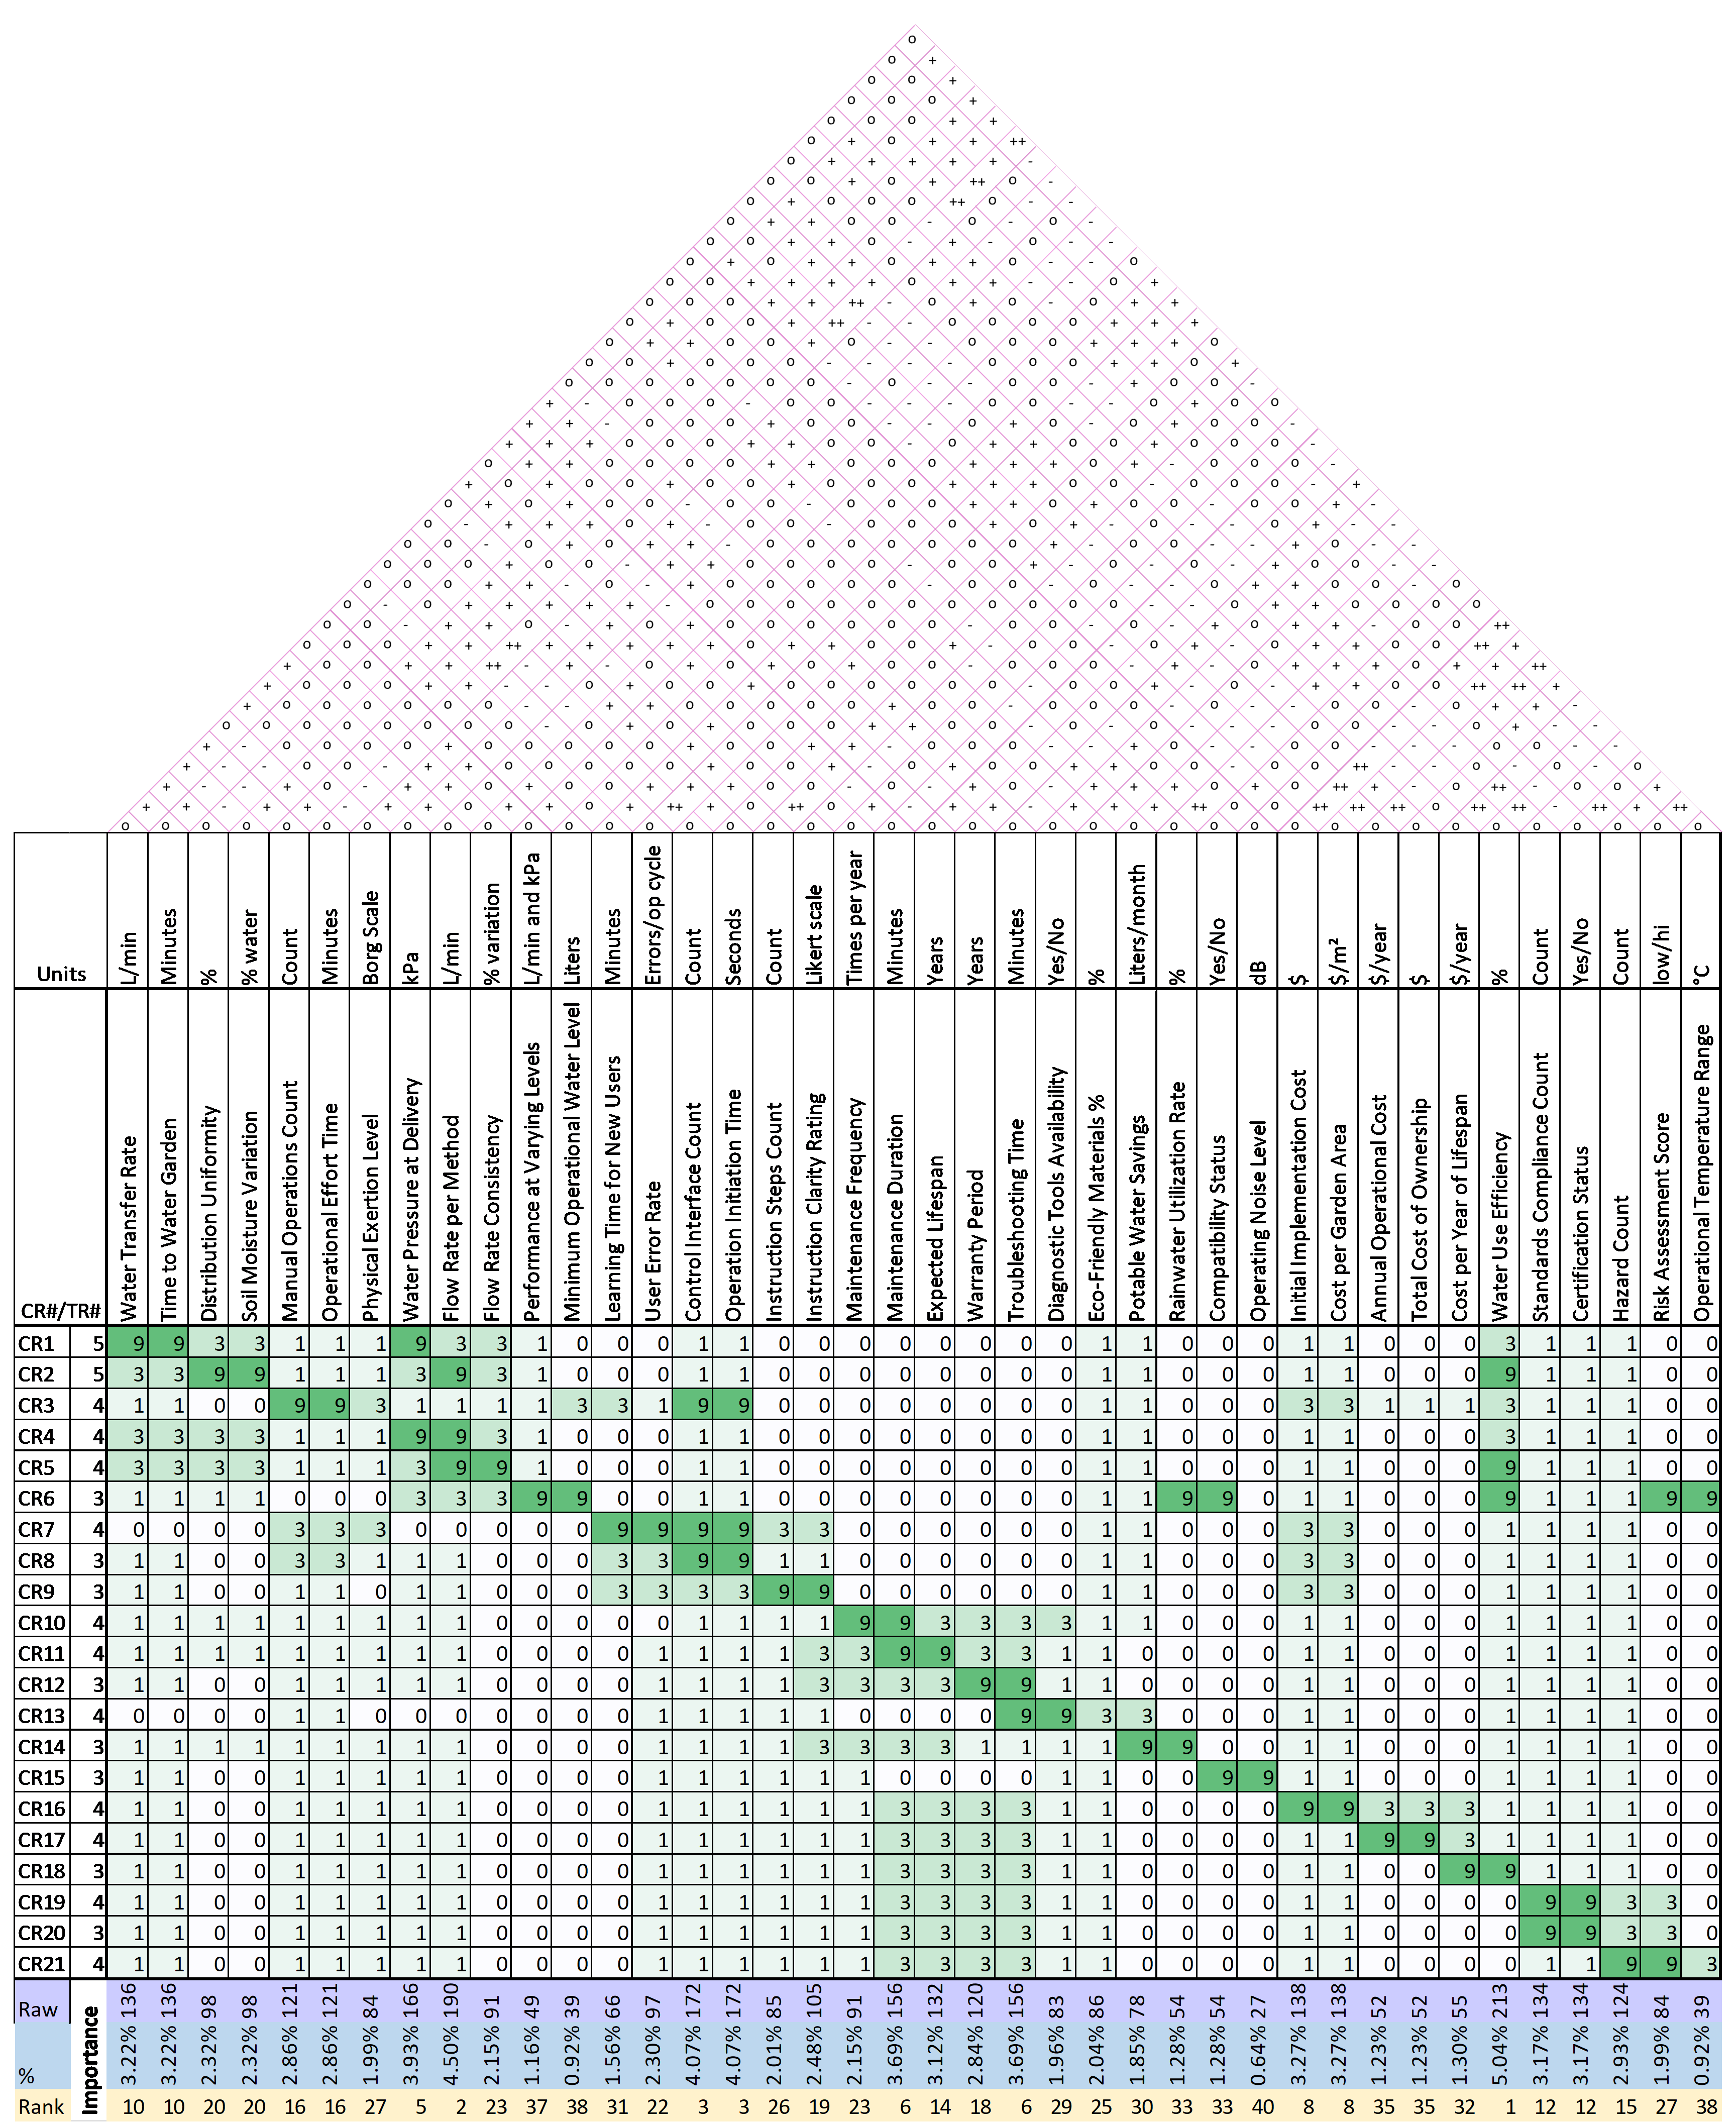
\includegraphics[width=\textwidth]{Roof_Relation_Importance.PNG}
    \caption{Correlation and Relationship Matrices with Importance Ranking}
    \label{figure:NeedsMetricsMatrix1}
\end{figure}

\subsubsection{Figure \ref{figure:NeedsMetricsMatrix1}: Correlation and Relationship Matrices with Importance Ranking}

Figure \ref{figure:NeedsMetricsMatrix1} displays the main components of the HoQ:

\begin{itemize}
    \item \textbf{Left Side (Customer Needs and Importance):} The customer needs are listed along the left side of the matrix, each assigned an Importance Factor (1-5). For example, "The system should provide sufficient water pressure" has an importance rating of 5.

    \item \textbf{Top (Engineering Characteristics):} The ECs are listed across the top of the matrix, including "Water Transfer Rate (L/min)," "Water Pressure (kPa)," and others.

    \item \textbf{Relationship Matrix (Central Grid):} The central grid shows the relationships between customer needs and ECs. Each cell contains a value (0, 1, 3, or 9) indicating the strength of the relationship. For instance, there is a strong relationship (9) between "The system should provide sufficient water pressure" and "Water Pressure (kPa)."

    \item \textbf{Correlation Matrix (Roof):} The triangular matrix at the top (the "roof") displays correlations between ECs. Positive correlations are marked with a "+", and negative correlations with a "-". For example, there is a negative correlation between "Water Pressure (kPa)" and "Energy Consumption (kWh)" indicating that increasing pressure may increase energy consumption.

    \item \textbf{Importance Ranking (Right Side):} The weighted importance of each EC is calculated and listed on the right side of the matrix. This helps prioritize the ECs based on their overall impact on customer needs.

\end{itemize}

\begin{figure}[h!]
    \centering
    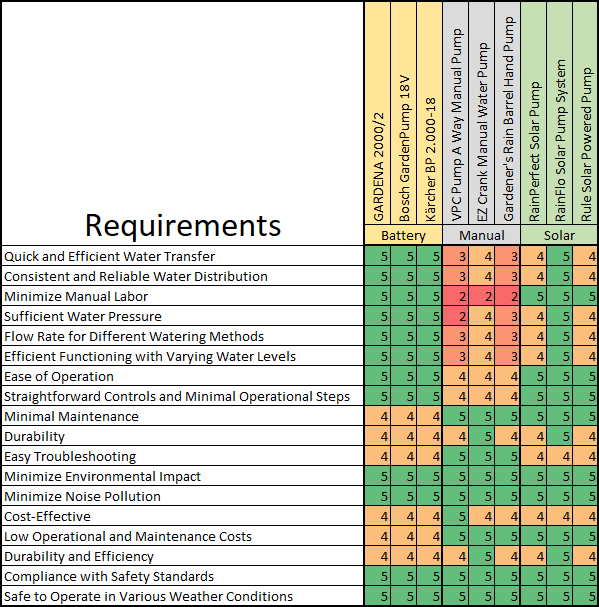
\includegraphics[width=\textwidth]{Competitor.PNG}
    \caption{Competitor Assessment}
    \label{figure:CompetitorAssessment}
\end{figure}

\subsubsection{Figure \ref{figure:CompetitorAssessment}: Competitor Assessment}

Figure \ref{figure:CompetitorAssessment} presents the benchmarking analysis against competitor products:

\begin{itemize}
    \item \textbf{Competitor Products Listed:} Products such as "Gardena 2000/2 Battery Pump," "Bosch GardenPump 18V," and "VPC Pump A Way Manual Pump" are listed.

    \item \textbf{Performance Ratings:} The performance of each competitor on the customer needs is rated on a scale (e.g., 1-5). For example, battery-powered pumps score higher on "Ease of Use" compared to manual pumps.

\end{itemize}

\subsubsection{Interpreting the Figures}

These figures provide a visual tool for analyzing how well the proposed system and competitor products meet the customer needs, and which ECs are most critical for success. By examining the relationship and correlation matrices, key areas of focus and potential conflicts that need to be addressed in the design can be identified.

\subsection{Observations and Analysis}

Based on the Needs Metrics Matrix, several critical insights were identified:

\begin{itemize}
    \item \textbf{High Impact Customer Needs:}

    The customer need "The system should provide sufficient water pressure" has the highest importance rating (5) and strong relationships (9) with multiple ECs, including "Water Pressure (kPa)" and "Water Transfer Rate (L/min)." This indicates that achieving adequate water pressure is paramount and will significantly influence the design.

    \item \textbf{Engineering Characteristics with Multiple Strong Relationships:}

    "Water Pressure (kPa)" and "Water Transfer Rate (L/min)" are ECs that have strong relationships with several high-importance customer needs. For example, "Water Pressure (kPa)" is strongly related (9) to both "The system should provide sufficient water pressure" and "The system should distribute water consistently," both rated with high importance. This highlights these ECs as critical focus areas in the design.

    \item \textbf{Trade-offs Identified in Correlation Matrix:}

    The correlation matrix reveals a negative correlation between "Water Pressure (kPa)" and "Energy Consumption (kWh)." Increasing water pressure may lead to higher energy consumption, which conflicts with the customer need to "Minimize operational cost," also rated with high importance (4). This trade-off necessitates exploring energy-efficient pump technologies or alternative solutions to balance these requirements.

    \item \textbf{Overlapping Metrics Indicating Complexity:}

    The customer need "The system should be easy to use" is measured by multiple metrics, including "Learning Time (hours)" and "User Error Rate (\%)." These metrics have strong relationships with ECs such as "Control Interface Count" and "Operation Initiation Time (seconds)." The overlapping metrics suggest that designing for usability will require careful consideration of user interface design and operational simplicity.

    \item \textbf{Sustainability Considerations:}

    Environmental impact is a significant concern, with customer needs such as "The system should have minimal environmental impact" rated with high importance (5). ECs like "Potable Water Savings (liters/month)" and "Eco-Friendly Materials (\%)" are crucial for meeting these needs. The positive correlation between "Potable Water Savings" and "Rainwater Utilization Rate (\%)" indicates an opportunity to enhance sustainability by maximizing rainwater usage.

    \item \textbf{Competitor Performance Gaps:}

    Competitor assessment shows that battery-powered pumps perform well in "Ease of Use" and "Water Transfer Rate" but may fall short in "Minimizing Environmental Impact." Manual pumps are cost-effective but perform poorly in "Minimizing Manual Labor" and "Water Transfer Rate." This suggests a market opportunity for a system that combines high performance with environmental sustainability.

\end{itemize}

\subsection{Key Trade-offs in Engineering Characteristics}

Designing the Rain Barrel Water Pump System involves balancing several competing engineering characteristics due to inherent trade-offs:

\begin{itemize}
    \item \textbf{Water Pressure vs. Energy Consumption:}

    Achieving higher water pressure and flow rates typically requires more powerful pumps, which increases energy consumption. This conflicts with the customer need to "Minimize operational cost" and "The system should be energy efficient." To address this trade-off, energy-efficient pump technologies, variable speed drives, or alternative energy sources such as solar power need to be considered to maintain high performance without significantly increasing energy usage.

    \item \textbf{Automation vs. Complexity and Cost:}

    Incorporating automation features (e.g., automatic start/stop, timers) enhances ease of use and reduces manual labor but adds complexity and cost to the system. This trade-off requires evaluating the value added by automation against budget constraints and potential maintenance challenges. Selecting reliable, cost-effective automation components will be critical.

    \item \textbf{Material Durability vs. Environmental Impact:}

    Using durable materials like certain plastics may improve system longevity but may not align with environmental sustainability goals if the materials are not eco-friendly. Conversely, eco-friendly materials may have shorter lifespans or higher costs. This trade-off necessitates careful material selection to balance durability, environmental impact, and cost.

    \item \textbf{Noise Reduction vs. Cost:}

    Reducing operational noise enhances user comfort and aligns with the need "The system should minimize noise pollution," but may require additional components like noise dampeners or quieter, more expensive pumps. Evaluating whether the benefits justify the increased cost is necessary.

    \item \textbf{System Complexity vs. Ease of Maintenance:}

    A more complex system may offer better performance or features but could be harder to maintain. This conflicts with the need for "The system should be easy to maintain." Simplifying the design where possible can improve maintainability but may limit functionality.

\end{itemize}

Understanding these trade-offs is essential for making informed design decisions that align with customer priorities while acknowledging practical limitations.

\newpage
\section{Target and Fallback Specifications}

\subsection{Explanation of Process}

\begin{itemize}
    \item \textbf{Data Collection:} Specifications of competitive products (solar, manual, battery-powered pumps) were reviewed. Data were referenced from multiple sources (see Table \ref{tab:TargetFallback}, e.g., A.1, B.2, etc.).

    \item \textbf{Target Values:} Established by averaging top-performing products and aligning with customer needs. For example, battery-powered pumps set the "Water Transfer Rate" target (50--60 L/min); fallback for solar-powered systems (30--49 L/min).

    \item \textbf{Fallback Values:} Derived from lower-performing systems or potential failure scenarios. Calculations based on competitor data and technical analyses (details in Appendix A).

    \item \textbf{Assumptions:} Some values, like "Operational Temperature Range," were assumed based on environmental conditions typical for the USC campus (-5°C to 40°C).

    \item \textbf{References:} Each value in Table \ref{tab:TargetFallback} is cited with proper references from product data, standards, or calculations.

\end{itemize}

\subsection{Product Target and Fallback Values}

Table \ref{tab:TargetFallback} provides a summary of product requirements, including target and fallback ranges for each Engineering Characteristic (EC). All values are backed by competitor data, industry standards, or calculations, with detailed references in Appendix A for validation (e.g., A.1, B.1, etc.).

\begin{table}[H!]
\centering
    \caption{Target, Fallback, and Competitor Ranges}
    \label{tab:TargetFallback}
    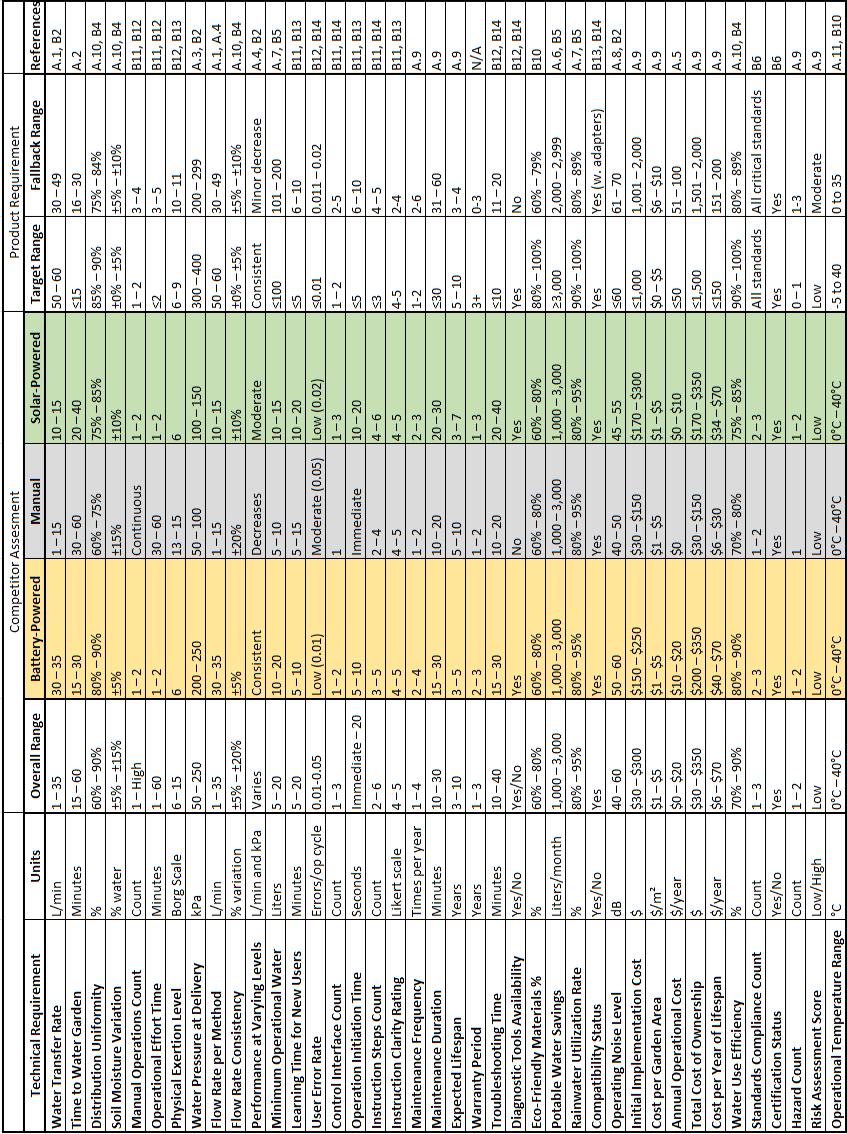
\includegraphics[width=\textwidth]{ranges.PNG}
\end{table}

\newpage
\section{Conclusions}

The House of Quality analysis provided critical insights into the design priorities and challenges for the Rain Barrel Water Pump System. The most impactful engineering characteristics identified are:

\begin{itemize}
    \item \textbf{Water Transfer Rate (L/min)} and \textbf{Water Pressure (kPa)}: These are essential for effective irrigation and meeting the high-importance customer need for sufficient water pressure. Achieving the target specifications of 50--60 L/min flow rate and 300--400 kPa pressure is challenging due to potential increases in energy consumption and cost.

    \item \textbf{Energy Consumption (kWh)}: Minimizing energy usage is crucial to meet operational cost targets and environmental goals. Balancing this with the need for high water pressure requires innovative solutions, such as energy-efficient pumps or alternative energy sources.

    \item \textbf{Ease of Use Metrics}: "Operational Effort Time" and "User Error Rate" are critical for ensuring the system is user-friendly. Designing intuitive controls and minimizing manual operations are necessary but may add complexity and cost.

    \item \textbf{Environmental Impact Metrics}: Maximizing "Potable Water Savings" and "Rainwater Utilization Rate" align with sustainability goals. However, achieving high utilization rates depends on environmental factors like rainfall patterns, which may be beyond control.

\end{itemize}

\subsection{Most Challenging Specifications}

The most challenging specifications to satisfy are:

\begin{itemize}
    \item \textbf{High Water Pressure with Low Energy Consumption}: Achieving the target water pressure without significantly increasing energy consumption requires careful selection of pump technology and potential use of energy recovery or renewable energy sources.

    \item \textbf{Automation Features within Budget Constraints}: Incorporating automation to minimize operational effort and user error must be balanced against cost limitations. Identifying cost-effective solutions or modular designs that allow for future upgrades may be necessary.

    \item \textbf{Material Selection for Durability and Sustainability}: Selecting materials that are both durable and environmentally friendly is challenging due to potential cost implications and availability of suitable materials.

\end{itemize}

\subsection{Influence on Future Design Decisions}

The findings from the HoQ analysis will guide future design decisions by:

\begin{itemize}
    \item \textbf{Prioritizing Critical ECs}: Focusing design efforts on optimizing water pressure and flow rate while exploring energy-efficient solutions.

    \item \textbf{Exploring Innovative Technologies}: Investigating alternative pump technologies, such as variable frequency drives or solar-powered pumps, to address trade-offs between performance and energy consumption.

    \item \textbf{Balancing Cost and Functionality}: Evaluating the cost-benefit of automation features and material choices to ensure the system meets customer needs without exceeding budget constraints.

    \item \textbf{Engaging Stakeholders}: Continuing to collaborate with USC Facilities and end-users to refine requirements and ensure that design decisions align with their priorities and expectations.

\end{itemize}

\subsection{Next Steps}

Moving forward, the design team will:

\begin{itemize}
    \item Develop concept designs that address the critical ECs and trade-offs identified.
    \item Perform detailed technical analyses and simulations to validate potential solutions.
    \item Prepare prototypes for testing key functionalities, particularly related to water pressure and energy consumption.
    \item Continue to update and refine the HoQ as more data becomes available and as design iterations progress.

\end{itemize}

\newpage
\appendix

\section{Appendix A: Calculations}

\subsection{Water Transfer Rate and Time to Fill Water Can}

To determine the target and fallback ranges for the water transfer rate and the time to fill a 2-gallon (7.57 liters) water can, perform the following calculations.

\subsubsection{Target Calculation:}

Desired fill time for the water can is 10 seconds.

\[
\text{Required Flow Rate}_{\text{target}} = \frac{\text{Volume of Can}}{\text{Desired Fill Time}} = \frac{7.57\ \text{liters}}{10\ \text{seconds}} = 0.757\ \text{L/s} = 45.42\ \text{L/min}
\]

\noindent To ensure efficient operation and account for potential system losses, set the target flow rate between \textbf{50 and 60 L/min}.

\subsubsection{Fallback Calculation:}

Acceptable fill time is up to 30 seconds.

\[
\text{Required Flow Rate}_{\text{fallback}} = \frac{7.57\ \text{liters}}{30\ \text{seconds}} = 0.252\ \text{L/s} = 15.14\ \text{L/min}
\]

\noindent Considering practical limitations and the need for efficiency, set the fallback flow rate between \textbf{30 and 49 L/min}.

\subsection{Total Time to Water Garden and Required Pump Flow Rate}

Assuming the garden requires a total volume of water and the desired total watering time.

\subsubsection*{Assumptions:}
\begin{itemize}
\item Total water needed per watering session: \( V_{\text{garden}} = 500\ \text{liters} \)
\item Desired total watering time (target): \( T_{\text{target}} = 15\ \text{minutes} \)
\item Acceptable total watering time (fallback): \( T_{\text{fallback}} = 30\ \text{minutes} \)
\end{itemize}

\subsubsection{Target Calculation:}

Required pump flow rate to meet target time:

\[
Q_{\text{target}} = \frac{V_{\text{garden}}}{T_{\text{target}}} = \frac{500\ \text{liters}}{15\ \text{minutes}} = 33.33\ \text{L/min}
\]

Since this flow rate is less than the flow rate calculated in A.1, a pump capable of delivering \textbf{50–60 L/min} will meet and exceed this requirement, ensuring faster watering if needed.

\subsubsection{Fallback Calculation:}

Required pump flow rate to meet fallback time:

\[
Q_{\text{fallback}} = \frac{500\ \text{liters}}{30\ \text{minutes}} = 16.67\ \text{L/min}
\]

This flow rate falls within the fallback range from A.1, ensuring acceptable performance if higher flow rates are not achievable.

\subsection{Water Pressure at Delivery and Sprinkler Operation}

To achieve the client's preference for high pressure sufficient to run a sprinkler, calculate the required water pressure.

\subsubsection*{Assumptions:}

\begin{itemize}
\item Standard sprinkler operating pressure: \( P_{\text{sprinkler}} = 275\ \text{kPa} \) (approximately 40 psi)
\item Desired pressure at delivery (target): \( P_{\text{target}} = 300\ \text{kPa} \) to \( 400\ \text{kPa} \)
\item Acceptable pressure at delivery (fallback): \( P_{\text{fallback}} = 200\ \text{kPa} \) to \( 299\ \text{kPa} \)
\end{itemize}

\subsubsection{Calculation:}

Given the tank is located 5 ft (1.524 m) above the garden level, can calculate the static pressure contribution due to elevation:

\[
P_{\text{elevation}} = \rho g h = 1000\ \text{kg/m}^3 \times 9.81\ \text{m/s}^2 \times 1.524\ \text{m} = 14,951\ \text{Pa} = 14.95\ \text{kPa}
\]

This static pressure is insufficient to operate a sprinkler; thus, a pump must provide additional pressure.

\subsubsection*{Total Required Pump Pressure:}

\[
P_{\text{pump}} = P_{\text{sprinkler}} - P_{\text{elevation}} = 275\ \text{kPa} - 14.95\ \text{kPa} = 260.05\ \text{kPa}
\]

To account for friction losses and ensure adequate pressure, target a pump pressure between \textbf{300 and 400 kPa}.

\subsection{Pump Power Requirement and Selection}

Determining the required pump power to achieve the target flow rate and pressure.

\begin{itemize}
\item Target flow rate: \( Q = 50\ \text{L/min} = 0.000833\ \text{m}^3/\text{s} \)
\item Target pressure increase: \( P = 300\ \text{kPa} \)
\end{itemize}

\subsubsection*{Hydraulic Power Calculation:}

\[
P_{\text{hydraulic}} = P \times Q = 300,000\ \text{Pa} \times 0.000833\ \text{m}^3/\text{s} = 249.9\ \text{W}
\]

\subsubsection*{Accounting for Efficiency:}

Assuming a pump efficiency \( \eta = 60\% \):

\[
P_{\text{input}} = \frac{P_{\text{hydraulic}}}{\eta} = \frac{249.9\ \text{W}}{0.6} = 416.5\ \text{W}
\]

Therefore, a pump with an input power of at least \textbf{500 W} is required to meet the target specifications.

\subsection{Energy Consumption and Annual Operational Cost}

Estimating the annual energy consumption and operational cost.

\subsubsection*{Assumptions:}

\begin{itemize}
\item Operating time per session: 15 minutes (0.25 hours)
\item  Number of sessions per week: 5
\item Weeks per year: 52
\item Pump input power: 500 W (0.5 kW)
\item Electricity cost: \$0.15 per kWh
\end{itemize}

\subsubsection*{Total Operating Hours per Year:}

\[
\text{Total Hours} = 0.25\ \text{hours/session} \times 5\ \text{sessions/week} \times 52\ \text{weeks/year} = 65\ \text{hours/year}
\]

\subsubsection*{Annual Energy Consumption:}

\[
\text{Energy} = \text{Power} \times \text{Total Hours} = 0.5\ \text{kW} \times 65\ \text{hours} = 32.5\ \text{kWh/year}
\]

\subsubsection*{Annual Operational Cost:}

\[
\text{Cost} = \text{Energy} \times \text{Electricity Rate} = 32.5\ \text{kWh/year} \times \$0.15/\text{kWh} = \$4.88\ \text{per year}
\]

\noindent This cost is well within the target of \(\leq\$50\) per year.

\subsection{Potable Water Savings Calculation}

Calculating the amount of potable water saved by using the rainwater system.

\subsubsection*{Assumptions:}

\begin{itemize}
\item Total water usage per week: \( 500\ \text{liters/session} \times 5\ \text{sessions/week} = 2,500\ \text{liters/week} \)
\item Weeks per month (average): 4.33
\end{itemize}

\subsubsection*{Monthly Water Savings:}

\[
\text{Monthly Savings} = 2,500\ \text{liters/week} \times 4.33\ \text{weeks/month} = 10,825\ \text{liters/month}
\]

This exceeds the target potable water savings of \(\geq3,000\) liters per month.

\subsection{Rainwater Utilization Rate and Tank Capacity Analysis}

Analyzing tank capacity and utilization rate.

\subsubsection*{Tank Capacity:}

- Tank capacity: 1,000 gallons = 3,785 liters

\subsubsection*{Monthly Water Demand:}

- From A.6: 10,825 liters/month

\subsubsection*{Number of Tank Refills Needed:}

\[
\text{Refills} = \frac{\text{Monthly Demand}}{\text{Tank Capacity}} = \frac{10,825\ \text{liters}}{3,785\ \text{liters}} \approx 2.86
\]

\subsubsection*{Utilization Rate Calculation:}

If the tank is refilled by rain at least 3 times per month, the rainwater utilization rate is:

\[
\text{Utilization Rate} = \frac{\text{Rainwater Used}}{\text{Total Water Demand}} \times 100\% = \frac{10,825\ \text{liters}}{10,825\ \text{liters}} \times 100\% = 100\%
\]

If refills are less frequent due to insufficient rainfall, utilization rate decreases.

\subsubsection*{Target:} Achieve a utilization rate of \textbf{90–100\%}.


\subsection{Noise Level Calculation}
Noise level attenuation over distance can be estimated using the inverse square law for sound:

\begin{equation}
    L_2 = L_1 - 20 \log \left( \frac{d_2}{d_1} \right)
\end{equation}

where:
\begin{itemize}
    \item $L_2$ is the noise level at the target distance,
    \item $L_1$ is the initial noise level (dB),
    \item $d_1$ is the initial distance from the source (m),
    \item $d_2$ is the target distance from the source (m).
\end{itemize}

For a system where the initial noise level at 1 meter is 50 dB, and want to estimate the noise level at 5 meters:

\[
L_2 = 50 - 20 \log \left( \frac{5}{1} \right) = 50 - 20 \log 5 \approx 36 \, \text{dB}
\]

Thus, at 5 meters, the noise level is reduced to approximately 36 dB.

\subsection{Total Cost of Ownership Over Lifespan}

Calculating total cost over expected lifespan, including initial and operational costs.

\subsubsection*{Assumptions:}

\begin{itemize}
    \item Initial implementation cost (target): \(\leq\$1,000\)
\item Expected lifespan: 5 years (minimum target)
\item Annual operational cost: \$50 (from A.5)
\item Maintenance cost: Minimal, included in operational cost
\end{itemize}

\subsubsection*{Total Cost Calculation:}

\[
\text{Total Cost}_{\text{target}} = \text{Initial Cost} + (\text{Annual Operational Cost} \times \text{Lifespan}) = \$1,000 + (\$50 \times 5) = \$1,250
\]

\subsubsection*{Cost per Year of Lifespan:}

\[
\text{Cost per Year} = \frac{\text{Total Cost}}{\text{Lifespan}} = \frac{\$1,250}{5\ \text{years}} = \$250\ \text{per year}
\]

\noindent This exceeds the target of \(\leq\$150\) per year. To meet the target:

\noindent If the initial cost is reduced to \$750:

\[
\text{Total Cost} = \$750 + (\$50 \times 5) = \$1,000
\]
\[
\text{Cost per Year} = \frac{\$1,000}{5\ \text{years}} = \$200\ \text{per year}
\]

Still above the target; further reduction needed.

\noindent If lifespan is extended to 10 years:

\[
\text{Total Cost} = \$1,000 + (\$50 \times 10) = \$1,500
\]
\[
\text{Cost per Year} = \frac{\$1,500}{10\ \text{years}} = \$150\ \text{per year}
\]

Meets the target cost per year. Thus, To achieve the target cost per year, the system should be designed for a lifespan of at least \textbf{10 years}.

\subsection{Water Use Efficiency and Distribution Uniformity}

Calculating water use efficiency (WUE) and distribution uniformity (DU).

\begin{itemize}
    \item Water Use Efficiency (WUE): The ratio of water beneficially used to the total water applied.
\item Distribution Uniformity (DU): A measure of how uniformly water is applied over the area.
\end{itemize}

\noindent
\textbf{Target for WUE:} \(\geq90\%\)

\noindent
\textbf{Target for DU:} 85–90\%

\noindent

Assuming the irrigation system has low losses (minimal runoff, evaporation, etc.), and high DU due to proper sprinkler operation. DU is calculated using the lowest quarter distribution method:

\[
\text{DU} = \frac{\text{Average of Lowest Quartile Catch Measurements}}{\text{Average of All Catch Measurements}} \times 100\%
\]

Assuming measurements support a DU of 88\% (within target range). If DU is high and system losses are low:

\[
\text{WUE} = \text{DU} - \text{Losses}
\]

Assuming losses are 5\%:

\[
\text{WUE} = 88\% - 5\% = 83\%
\]

This falls into the fallback range of \(\geq80\%\). To meet the target WUE of \(\geq90\%\), losses must be reduced.

Implementing measures such as Using low-evaporation sprinklers, Scheduling irrigation during low wind and cooler temperatures, and Regular maintenance to prevent leaks may reduce losses.

By reducing losses to 2\%:

\[
\text{WUE} = 88\% - 2\% = 86\%
\]

Still within fallback range; further improvements needed.

\subsection{Operational Temperature Range and Material Selection}

Ensuring the system operates effectively within the required temperature range.

\subsubsection{Target Range:} \(-5^\circ\text{C}\) to \(40^\circ\text{C}\)

\subsubsection{Fallback Range:} \(0^\circ\text{C}\) to \(35^\circ\text{C}\)

\subsubsection*{Material Considerations:}

\begin{itemize}
    \item Components must withstand potential freezing temperatures (\(-5^\circ\text{C}\)).
\item Materials such as PVC pipes and fittings are suitable within this range.
\item Electrical components should be rated for outdoor use with appropriate temperature ratings.
\end{itemize}

Determine the coefficient of thermal expansion for materials to ensure structural integrity. For PVC:

\[
\text{Coefficient of Thermal Expansion} = 7 \times 10^{-5}\ \text{per }^\circ\text{C}
\]

Calculate length change (\( \Delta L \)) for a 10 m pipe over a temperature change (\( \Delta T \)) of 45°C (\(-5^\circ\text{C}\) to \(40^\circ\text{C}\)):

\[
\Delta L = L \times \text{Coefficient} \times \Delta T = 10\ \text{m} \times 7 \times 10^{-5}\ \text{per }^\circ\text{C} \times 45^\circ\text{C} = 0.0315\ \text{m} = 31.5\ \text{mm}
\]

Allowances must be made in the design to accommodate this expansion and contraction.


\appendix

\section{Appendix B: References}

\begin{thebibliography}{9}

\bibitem{IrrigationEngineering}
Jensen, M. E., Burman, R. D., \& Allen, R. G. (1990). \emph{Evaporation, Evapotranspiration, and Irrigation Water Requirements}. American Society of Civil Engineers.

\bibitem{PumpHandbook}
Karassik, I. J., Krutzsch, W. C., Fraser, W. H., \& Messina, J. P. (2001). \emph{Pump Handbook} (3rd ed.). McGraw-Hill.

\bibitem{FluidMechanics}
Munson, B. R., Young, D. F., \& Okiishi, T. H. (2013). \emph{Fundamentals of Fluid Mechanics} (7th ed.). Wiley.

\bibitem{IrrigationSystems}
Hoffman, G. J., Evans, R. G., Jensen, M. E., Martin, D. L., \& Elliott, R. L. (2007). \emph{Design and Operation of Farm Irrigation Systems} (2nd ed.). American Society of Agricultural and Biological Engineers.

\bibitem{RainwaterHarvesting}
Gould, J., \& Nissen-Petersen, E. (1999). \emph{Rainwater Catchment Systems for Domestic Supply: Design, Construction and Implementation}. Intermediate Technology Publications.

\bibitem{HydraulicEngineering}
Chadwick, A., \& Morfett, J. (2013). \emph{Hydraulics in Civil and Environmental Engineering} (5th ed.). CRC Press.

\bibitem{EnvironmentalEngineering}
Mihelcic, J. R., \& Zimmerman, J. B. (2014). \emph{Environmental Engineering: Fundamentals, Sustainability, Design} (2nd ed.). Wiley.

\bibitem{WaterResources}
Mays, L. W. (2010). \emph{Water Resources Engineering} (2nd ed.). Wiley.

\bibitem{GreenInfrastructure}
Fletcher, T. D., Shuster, W., Hunt, W. F., et al. (2015). \emph{SUDS, LID, BMPs, WSUD and More – The Evolution and Application of Terminology Surrounding Urban Drainage}. Urban Water Journal, 12(7), 525–542.

\bibitem{SustainableMaterials}
Ashby, M. F. (2012). \emph{Materials and the Environment: Eco-informed Material Choice} (2nd ed.). Butterworth-Heinemann.

\bibitem{DesignEverydayThings}
Norman, D. A. (2013). \emph{The Design of Everyday Things} (Revised and Expanded Edition). Basic Books.

\bibitem{HumanFactors}
Sanders, M. S., \& McCormick, E. J. (1993). \emph{Human Factors in Engineering and Design} (7th ed.). McGraw-Hill.

\bibitem{ProductDesign}
Ulrich, K. T., \& Eppinger, S. D. (2015). \emph{Product Design and Development} (6th ed.). McGraw-Hill Education.

\bibitem{HumanFactorsHandbook}
Salvendy, G. (Ed.). (2012). \emph{Handbook of Human Factors and Ergonomics} (4th ed.). Wiley.

\bibitem{EngineeringPsychology}
Wickens, C. D., Gordon, S. E., \& Liu, Y. (1998). \emph{An Introduction to Human Factors Engineering}. Longman.

\end{thebibliography}

\end{document}